\documentclass[11pt,a4paper]{article}
\usepackage{ls}
\usepackage[german]{babel}

\title{Themen für Seminararbeiten\\ im Modul \emph{Angewandte Informatik}\\ im
  Wintersemester 2020/21}

\author{Hans-Gert Gr\"abe}

\date{26. Januar 2021}

\begin{document}
\maketitle

\section{Hintergrund}

Im Bereich der TRIZ-Forschung wurde vor einem Jahr das \emph{TRIZ Summit
  Ontologie-Projekt}\footnote{Siehe \url{https://triz-summit.ru/onto_triz/}
  (in Russisch).}  begonnen, um die verschiedenen Teile der TRIZ-Theorie
ontologisch zu „kartieren“ und die wesentlichen Zusammenhänge zwischen den
einzelnen Teilen mit Mitteln semantischer Technologien zu erfassen. Hierzu
liegen aktuell vor
\begin{itemize}[noitemsep]
\item[(1)] eine „Übersichtskarte“ der verschiedenen Theoriefelder und der
  Zusammenhänge zwischen diesen,
\item[(2)] ein „Atlas“ von Ontokarten, die grob einzelne Bereiche markieren,
  die weiter zu detaillieren sind,
\item[(3)] zu einzelnen dieser Ontokarten erste Versuche, Struktur in das
  begriff\-liche Chaos zu bringen,
\item[(4)] ein Glossar (oder auch nur ein Thesaurus) von Begriffen, die
  hierfür wichtig sind.
\end{itemize}

Während zu (1) und (2) weitgehend Konsens besteht, sind die Modellierungen in
(3) stark umstritten, da die entsprechenden Semantiken und Zusammenhänge in
den unterschiedlichen TRIZ-Schulen naturgemäß unterschiedlich verstanden
werden.

Streit gibt es auch zu (4), der aber deutlich einfacher zu klären ist, wenn 
\begin{itemize}[noitemsep]
\item[(4a)] zunächst einmal alle Begriffe gesammelt und „URIfiziert“ werden
  (Thesaurus raw),
\item[(4b)] URIs so weit zusammengeführt werden, dass verschiedene URIs auf
  verschiedene Konzepte verweisen, aber Raum bleibt, für gleiche Konzepte
  verschiedene Semantiken zu hinterlegen (Thesaurus final),
\item[(4c)] diese verschiedenen Semantiken auch wirklich zusammengetragen und
  formalisiert werden (Glossar raw) und schließlich
\item[(4d)] die Semantiken in einem komplexen sozialen Abstimmungsprozess so
  weit wie \emph{möglich} abgeglichen und essenzielle Differenzen semantisch
  modelliert werden. 
\end{itemize}
In \cite{Kuryan2019} wird das Projekt genauer beschrieben, in
\cite{Kuryan2020} der aktuelle Stand dargestellt. Andere Vorarbeiten fanden
wenig Berücksichtigung\footnote{Details dazu auf der Webseite
  \url{https://wumm-project.github.io/Ontology.html}.}, insbesondere weder
\cite{IDM2011} noch \cite{GSA} oder \cite{VDI}. Im Herbst 2020 lief eine
Webinarreihe (in Russisch), deren Materialien auch verfügbar\footnote{Siehe
  \url{https://wumm-project.github.io/OntologyWebinar}.} und teilweise ins
Englische übersetzt sind.

Arbeitsgrundlage der TRIZ Summit Ontologie-Projekts ist ein Glossar von
V. Souchkov \cite{SG}, wobei dessen Einträge sowohl drei TRIZ-Generationen
(TRIZ-1..3) als auch 5 Kategorien (Basisbegriffe, Modelle, Regeln,
Begriffsgruppen, Synonyme) zugeordnet werden. Ein Webinarteilnehmer wies auf
einen weiteren Thesaurus \cite{GSA} auf den einschlägigen russischen
Altschullerseiten hin, der bereits multilingual vorliegt.

Im Rahmen des WUMM-Projekts wurden und werden Teile dieser Ontologisierungen
nachmodelliert und im \emph{WUMM RDFData github Repo}\footnote{Siehe dazu das
  Verzeichnis \texttt{Ontologies} im github-Repo
  \url{https://github.com/wumm-project/RDFData}} hochgeladen, die im Original
bisher ausschließlich durch grafische Ontogramme sowie die Möglichkeit einer
visuellen Inspektion im verwendeten OSA-Ontologie-Editor\footnote{Siehe
  \url{https://onto.devtas.ru/ts2o1} (in Russisch).} zugänglich sind.  Diese
im Original ausschließlich russischsprachigen Quellen wurden dabei in Teilen
auch ins Englische und Deutsche übertragen.  Weitgehend semantisch erfasst
sind (1) und (2). Weiterhin wurde bereits früher das VDI-Glossar „RDFiziert“
und die dort vorhandenen deutschen und englischen Erläuterungen um eine
russische Übersetzung ergänzt. Dies sowie der einfach zu transformierende
Thesaurus auf den Altschullerseiten bilden die Grundlage für einen eigenen
Thesaurus nach (4a), der mit den Begriff\-lichkeiten des Originalprojekts
weiter abzugleichen ist.  Inzwischen wurde auch das Glossar \cite{SG} in der
aktuellen Version 1.2 auf diese Weise aufbereitet.  Details dazu weiter unten.

\section{Themen für Seminararbeiten}

In den Seminararbeiten soll am Punkt (3) weitergearbeitet werden, indem für
eine konkrete Ontokarte $X$ (bzw. einen anderen konkreten
Modellierungszusammenhang im TRIZ-Kontext entsprechend den mündlichen
Absprachen)
\begin{itemize}[noitemsep]
\item[(A)] die Zusammenhänge für das WUMM-Projekt in RDF in einer gemeinsamen
  Rahmensetzung nachmodelliert werden sowie
\item[(B)] differierende Semantiken, Probleme und Widersprüche im Verständnis
  der modellierten TRIZ-Konzepte zusammengetragen und systematisiert werden.  
\end{itemize}
Während (A) primär einen ingenieur-technischen Charakter hat, erfordert (B)
stärker einen akademischen Zugang von Recherche und Vergleich einschlägiger
Publikationen.

Informationen zu (A) liegen typischerweise in Form von RDF-Diagrammen vor, wie
etwa die \emph{Top Level Ontologie} in Abbildung 1, und sollen in eine
Turtle-Datei vergleichbar zur Datei \texttt{TopLevel.ttl} im WUMM RDFData
github Repo überführt werden. 

\begin{center}
  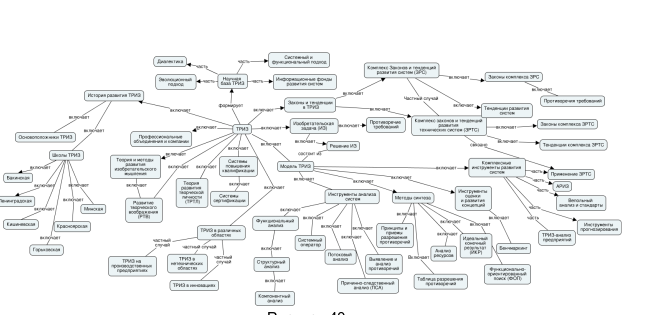
\includegraphics[width=\textwidth]{3.png}\\
  \textbf{Abbildung 1:} Die Top Level Ontologie als RDF Graph
\end{center}

Entsprechende Quellen für einen Startpunkt Ihrer Recherchen finden Sie in der
README-Datei in Ihrem Projektverzeichnis.

Für jede Seminararbeit ist ein Unterverzeichnis eingerichtet. Bitte forken Sie
(so weit noch nicht geschehen) das Repo auf einen eigenen Account, erstellen
die Seminararbeit und geben Zwischen- und das Endergebnis über einen
Merge-Request zur Begutachtung frei. Ich werde mich bemühen, die Ergebnisse
kurzfristig zu durchzusehen und mit Ihnen zu besprechen.

Die Seminararbeit selbst soll in {\LaTeX} erstellt werden und möglichst in
Englisch verfasst sein.

\section{Grundlagen des WUMM-Ontologie-Projekts}

Im TRIZ Summit Ontologie-Projekt geht es zunächst darum, die
TRIZ-Begriffslandschaft zu „kartieren“.  Das WUMM-Ontologie-Projekt begleitet
diese Aktivitäten, um
\begin{enumerate}[noitemsep]
\item eine Remodellierung nach semantischen Standards auszuführen,
\item die Materialien multilingual aufzubereitet und
\item auf dieser Basis eine LOD-Infrastruktur aufzubauen,
\end{enumerate}
und so eine bessere Basis für die erforderlichen sozialen Abstimmungsprozesse
zu schaffen.

\subsection{Die SKOS Ontologie als Basis}

Dafür wird die SKOS-Ontologie \cite{SKOS} verwendet, die mit den Konzepten (K)
\begin{itemize}[noitemsep]
\item \texttt{skos:Concept}, \texttt{skos:prefLabel}, \texttt{skos:altLabel}
  -- Objektbenennung
\item \texttt{skos:definition}, \texttt{skos:example}, \texttt{skos:note} --
  Objekteigenschaften
\item \texttt{skos:narrower}, \texttt{skos:broader} -- Objektrelationen
\end{itemize}
einen ersten Beschreibungsrahmen für Begrifflichkeiten bietet.  Für die
genauere Bedeutung der einzelnen Konzepte wird auf \cite{SKOS} veriesen.  Auf
der Basis wurden bisher drei Quellen ausgewertet,
\begin{itemize}[noitemsep]
\item der mehrsprachige Thesaurus \cite{GSA},
\item das Glossar der VDI-Norm \cite{VDI} und
\item das Glossar \cite{SG}, Version 1.2, von V. Souchkov.
\end{itemize}
Außerdem wurde das Glossar des TRIZ Summit Projekts teilweise integriert. Das
Glossar ist derzeit öffentlich nur in einer HTML-Veresion verfügbar. Interne
maschinenlesbare Versionen wurden mit dem Verweis auf den vorläufigen
Charakter der Modellierung noch nicht zur Veröffentlichung freigegeben.  Auch
lassen sich Daten in der OSA-Plattform nicht ohne Weiteres über eine API in
gängigen RDF-Formaten extrahieren. Deshalb habe ich den genaueren Abgleich
zugunsten der Konsolidierung des WUMM-Thesaurus zurückgestellt. 

\subsection{URIs und Namensräume}

Eines der zentralen Probleme der Überführung der vorhandenen Datenbestände zu
TRIZ-Konzepten ist die Zuweiseung sinnvoller URIs, da die einzelnen
Glossareinträge in den bisherigen Quellen einzig durch ihre Bezeichner
(„labels“) identifiziert werden.  Hier macht auch die OSA-Plattform keine
Ausnahme, denn die dort vergebenen URIs (sowohl für die Knoten als auch die
Kanten des aufgebauten RDF-Graphen) sind nach außen nicht sichtbar.

Bei der maschinellen Transformation der Datenbestände in ein valides
RDF-Format wurden automatisiert URIs erzeugt, die alle im Namensraum
\texttt{tc:} (wie \emph{TRIZ Concepts}) liegen. Eine wesentliche, noch
bevorstehende Aufgabe ist die Unifizierung der URIs aus den Quellen, also die
Zusammenführung von verschiedenen URIs, welche denselben Begriff bezeichnen.
Diese Arbeit soll demnächst in Angriff genommen werden. 

\subsection{Provenienz von Erläuterungen}

Ein wesentliches Problem dieser ontologischen Modellierung ist die genauere
Darstellung der Provenienz der einzelnen Erläuterungen. Hierzu wurden die
unter (K) aufgeführten SKOS-Konzepte für jede einzelne Quelle durch Notationen
aus dem Namensraum \texttt{od:} verfeinert, um zunächst die „Welten“ der
einzelnen Autoren und TRIZ-Schulen zu erfassen.

\texttt{od:} ist der Namensraum, den das WUMM-Projekt verwendet, um dort seine
eigenen Konzepte zu entwickeln.  Eine genauere Beschreibung dieses Namensraums
in einer eigenen RDF-Datei steht noch aus, die durch die URIs repräsentierten
Konzepte sind bisher nur mündlich abgestimmt.

Entsprechende Notationsvariationen sind etwa
\begin{itemize}[noitemsep]
\item \texttt{skos:Concept} $\to$ \texttt{od:GSAThesaurusEntry},
  \texttt{od:VDIGlossaryEntry} \ldots
\item \texttt{skos:definition} $\to$ \texttt{od:SouchkovDefinition},
  \texttt{od:VDIGlossaryDefinition} \ldots
\item \texttt{skos:example} $\to$ \texttt{od:VDIGlossaryExample} \ldots
\end{itemize}
usw. Siehe dazu die RDF-Daten selbst, die über den SPARQL-Endpunkt
\begin{center}
  \url{http://wumm.uni-leipzig.de:8891/sparql}
\end{center}
des WUMM-Projekts durchsucht werden können. Aus technischen Gründen tragen
alle Datensätze den RDF-Typ \texttt{skos:Concept}, auch wenn als 
\begin{center}
  \texttt{od:GSAThesaurusEntry} \texttt{rdfs:subClassOf} \texttt{skos:Concept}
\end{center}
diese Information inferiert werden könnte. 

\begin{thebibliography}{xxx}
\bibitem{IDM2011} D. Cavallucci, F. Rousselot, C. Zanni (2011). An ontology
  for TRIZ. Proc. TRIZ Future Conference 2009. Procedia Engineering 9,
  251–260.  \url{https://doi.org/10.1016/j.proeng.2011.03.116}.
\bibitem{Kuryan2019} A. Kuryan, V. Souchkov, D. Kucharavy (2019). Towards
  ontology of TRIZ. TRIZ Developers Summit, Minsk 2019.
  \\ \url{https://wumm-project.github.io/Texts/Ontology-TDS2019-en.pdf}
\bibitem{Kuryan2020} A. Kuryan, M. Rubin, N. Shchedrin, O. Eckardt, N. Rubina.
  TRIZ Ontology. Current State and Perspectives. TRIZ Developers Summit 2020
  (in Russisch). Englische Übersetzung:
  \\ \url{https://wumm-project.github.io/Texts/Ontology-TDS2020-en.pdf}
\bibitem{SG} V. Souchkov. Glossary of TRIZ and TRIZ-related terms. Mehrere
  Versionen seit 1991. Letzte Version 1.2 von 2014.
\bibitem{GSA} Thesaurus auf \texttt{altshuller.ru}.\\
  \url{https://www.altshuller.ru/thesaur/thesaur.asp}
\bibitem{VDI} VDI Richtlinie 4521. Erfinderisches Problemlösen mit TRIZ.\\
  Blatt 1: Grundlagen und Begriffe (April 2016).\\ Blatt 2: Zielbeschreibung,
  Problemdefinition und Lösungspriorisierung (April 2018).\\ Blatt 3:
  Lösungssuche (Juli 2020). 
\bibitem{SKOS} W3C (2008). SKOS Simple Knowledge Organization System RDF
  Schema.\\
  \url{https://www.w3.org/TR/2008/WD-skos-reference-20080829/skos.html}
\end{thebibliography}

\end{document}
